\subsection{Quản lý nghỉ phép}
\label{subsec:req_leave}
\label{subsec:module_leave}

\subsubsection{Mục tiêu và yêu cầu chức năng}

Ứng dụng hỗ trợ tra cứu quỹ phép tham khảo, lập đơn theo biểu mẫu ba bước, theo dõi và xử lý theo thẩm quyền. Kiểm tra ngày, số dư và xung đột trên mobile hỗ trợ hoàn thiện dữ liệu; backend HRM thực hiện kiểm tra nghiệp vụ cuối cùng và xử lý việc chuyển trạng thái hồ sơ.

\begin{table}[H]
\centering
\small
\caption{Yêu cầu chức năng nhóm quản lý nghỉ phép}
\label{tab:fr_leave}
\begin{tabularx}{\textwidth}{|L{1.8cm}|L{3.5cm}|L{2.5cm}|Y|}
\hline
\textbf{Mã FR} & \textbf{Chức năng} & \textbf{Tác nhân} & \textbf{Mô tả và ràng buộc nghiệp vụ} \\
\hline
FR-LEV-01 & Tra cứu quỹ phép và đơn & Nhân sự & Xem số dư quỹ phép năm tham khảo, lọc danh sách đơn theo năm và trạng thái xử lý. \\
\hline
FR-LEV-02 & Lập và gửi đơn nghỉ phép & Nhân sự & Nhập liệu theo biểu mẫu 3 bước, đính kèm minh chứng, lưu nháp hoặc gửi duyệt khi đáp ứng điều kiện nghiệp vụ. \\
\hline
FR-LEV-03 & Quản lý đơn đã tạo & Nhân sự & Chỉnh sửa hoặc xóa đơn ở trạng thái Nháp; chỉnh sửa và gửi lại đơn Bị trả lại. Đơn đã gửi không mặc định có thao tác thu hồi cho người lập. \\
\hline
FR-LEV-04 & Phê duyệt theo thẩm quyền & Cấp phê duyệt & Xem xét nội dung, minh chứng và phê duyệt, từ chối hoặc trả lại đơn theo thẩm quyền được phân công. \\
\hline
\end{tabularx}
\end{table}

Trong quy trình hiện thực, thao tác lưu giữ đơn ở trạng thái Nháp, còn thao tác gửi mới chuyển đơn sang bước chờ duyệt. Quyền thu hồi của người có thẩm quyền thuộc luồng xử lý riêng, không đồng nhất với quyền xóa đơn Nháp của người lập.

\subsubsection{Đặc tả Use Case}

UC-LEV-01 cụ thể hóa FR-LEV-01 và FR-LEV-03; UC-LEV-02 gắn với FR-LEV-02, còn UC-LEV-03 gắn với FR-LEV-04. Hình~\ref{fig:uc_leave} thể hiện các nhóm thao tác tương ứng.

\begin{figure}[H]
\centering
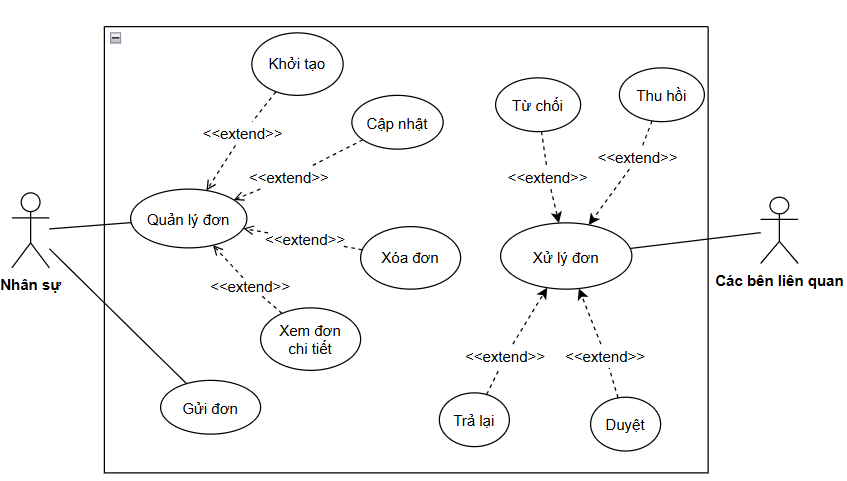
\includegraphics[width=\linewidth]{image/usecase/UC_LEAVE.png}
\caption{Sơ đồ Đặc tả Use case nhóm Quản lý nghỉ phép}
\label{fig:uc_leave}
\end{figure}

\usecasespec{
  id={UC-LEV-01},
  name={Quản lý đơn nghỉ phép cá nhân},
  shortname={Quản lý đơn cá nhân},
  actor={Nhân sự},
  desc={Cho phép nhân sự theo dõi số dư quỹ phép năm, tra cứu danh sách đơn và tiến trình duyệt; chỉnh sửa hoặc xóa đơn Nháp, chỉnh sửa và gửi lại đơn Bị trả lại.},
  pre={Nhân sự đã đăng nhập thành công vào ứng dụng MyHCMUT Mobile.},
  trigger={Người dùng chọn chức năng ``Nghỉ phép'' trên màn hình chính.},
  mainflow={
    1. Người dùng mở mục ``Nghỉ phép'' để xem số dư quỹ phép tham khảo và danh sách đơn đã lập. \newline
    2. Người dùng lọc danh sách hoặc chọn một đơn để xem trạng thái và tiến trình xử lý. \newline
    3. Với đơn Nháp, người dùng có thể tiếp tục chỉnh sửa hoặc xóa đơn. \newline
    4. HRM kiểm tra người lập và trạng thái đơn trước khi ghi nhận thao tác hợp lệ.
  },
  altflow={
    - \textit{Luồng 3a (Sửa đơn bị trả lại):} Với đơn ở trạng thái Bị trả lại, người dùng chọn chỉnh sửa để bổ sung thông tin và gửi lại. \newline
    - \textit{Luồng 3b (Theo dõi đơn đã gửi):} Với đơn đang chờ duyệt, người dùng xem trạng thái và lịch sử xử lý; ứng dụng không mặc định cung cấp thao tác thu hồi cho người lập.
  },
  exflow={
    - \textit{Ngoại lệ 4a (Trạng thái đã thay đổi):} Nếu đơn không còn ở trạng thái cho phép chỉnh sửa hoặc xóa, HRM từ chối thao tác và ứng dụng cập nhật trạng thái mới.
  },
  post={Nhân sự nắm bắt thông tin quỹ phép và trạng thái các đơn; những thay đổi hợp lệ đối với đơn Nháp hoặc đơn Bị trả lại được ghi nhận trên HRM.},
  label={tab:uc_lev_01}
}

\usecasespec{
  id={UC-LEV-02},
  name={Lập và gửi đơn nghỉ phép},
  shortname={Lập và gửi đơn nghỉ phép},
  actor={Nhân sự},
  desc={Cho phép nhân sự lập mới đơn nghỉ phép qua quy trình hướng dẫn 3 bước, kiểm tra thời gian và số dư phép, đính kèm minh chứng và gửi duyệt.},
  pre={Nhân sự đã đăng nhập vào hệ thống và có quyền lập đơn nghỉ phép.},
  trigger={Người dùng nhấn nút tạo mới đơn nghỉ phép trên giao diện ứng dụng.},
  mainflow={
    1. Người dùng chọn tạo mới đơn nghỉ phép; ứng dụng kiểm tra ngày đăng ký có hợp lệ trước khi yêu cầu tạo nháp. \newline
    2. Khi ngày đăng ký hợp lệ, hệ thống khởi tạo bản ghi nháp. \newline
    3. Người dùng nhập thông tin nghỉ phép và đính kèm minh chứng khi được yêu cầu. \newline
    4. Người dùng rà soát thông tin và gửi đơn. \newline
    5. HRM kiểm tra các điều kiện nghiệp vụ và tiếp nhận đơn hợp lệ vào quy trình chờ duyệt.
  },
  altflow={
    - \textit{Luồng 3a (Lưu nháp):} Người dùng chọn lưu nháp tại bất kỳ bước nào để tiếp tục hoàn thiện sau. \newline
    - \textit{Luồng 3b (Thoát biểu mẫu):} Người dùng xác nhận thoát; dữ liệu chưa lưu trên ứng dụng bị bỏ. Bản ghi nháp đã tạo trên HRM vẫn tồn tại, có thể mở lại hoặc xóa bằng thao tác riêng.
  },
  exflow={
    - \textit{Ngoại lệ 1a (Ngày đăng ký không hợp lệ):} Ứng dụng thông báo nguyên nhân và không tạo bản ghi nháp. \newline
    - \textit{Ngoại lệ 3a (Xung đột lịch trình):} Khoảng thời gian nghỉ trùng lặp với kế hoạch công tác hoặc đơn khác $\rightarrow$ hệ thống cảnh báo và yêu cầu điều chỉnh. \newline
    - \textit{Ngoại lệ 3b (Vượt số dư quỹ phép):} Số ngày đăng ký vượt quá số dư phép năm còn lại $\rightarrow$ hệ thống cảnh báo để người dùng điều chỉnh. \newline
    - \textit{Ngoại lệ 3c (Quá hạn đăng ký):} Khi kiểm tra thời hạn xác định không thể tạo đơn nghỉ phép thông thường, ứng dụng thông báo nguyên nhân và điều hướng người dùng đến điểm truy cập phân hệ Giải trình. Việc lập và xử lý Giải trình không thuộc phạm vi hiện thực của use case này.
  },
  post={Khi gửi thành công, đơn được ghi nhận ở bước chờ duyệt và phát sinh thông báo theo quy trình. Nếu chỉ lưu hoặc thoát sau khi tạo nháp, đơn vẫn ở trạng thái Nháp.},
  label={tab:uc_lev_02}
}

\usecasespec{
  id={UC-LEV-03},
  name={Xử lý đơn nghỉ phép},
  shortname={Xử lý đơn nghỉ phép},
  actor={Lãnh đạo Đơn vị, Chuyên viên Phòng Tổ chức Nhân sự, Ban Giám hiệu},
  desc={Cho phép người có thẩm quyền thẩm định nội dung đơn, kiểm tra tài liệu minh chứng và thực hiện phê duyệt, từ chối hoặc yêu cầu bổ sung thông tin.},
  pre={Người duyệt đã đăng nhập và đơn đang ở bước thuộc thẩm quyền xử lý của tài khoản.},
  trigger={Người duyệt mở danh sách đơn chờ xử lý từ ứng dụng hoặc qua thông báo nhắc việc.},
  mainflow={
    1. Người duyệt mở danh sách đơn nghỉ phép chờ xử lý thuộc thẩm quyền phân công. \newline
    2. Chọn xem chi tiết một đơn để kiểm tra nội dung và minh chứng liên quan. \newline
    3. Người duyệt lựa chọn hành động: \textit{Phê duyệt}, \textit{Từ chối} hoặc \textit{Trả lại}. \newline
    4. HRM kiểm tra quyền và trạng thái đơn hiện tại, rồi ghi nhận kết quả xử lý hoặc chuyển đơn sang bước tiếp theo. \newline
    5. Hệ thống thông báo kết quả cho nhân sự lập đơn; số dư phép được cập nhật khi đơn hoàn tất theo quy tắc nghiệp vụ.
  },
  altflow={
    - \textit{Luồng 3a (Xử lý đồng loạt):} Người duyệt chọn nhiều đơn hợp lệ trên danh sách và thực hiện phê duyệt hàng loạt. \newline
    - \textit{Luồng 3b (Trả lại yêu cầu chỉnh sửa):} Người duyệt chọn ``Trả lại'' kèm ý kiến yêu cầu $\rightarrow$ đơn chuyển sang trạng thái Bị trả lại để nhân sự hoàn thiện.
  },
  exflow={
    - \textit{Ngoại lệ 3a (Từ chối đơn):} Người duyệt bắt buộc nhập lý do từ chối trước khi hệ thống ghi nhận kết quả. \newline
    - \textit{Ngoại lệ 4a (Trạng thái không phù hợp):} Khi HRM xác định đơn không còn ở bước cho phép xử lý, thao tác bị từ chối và người dùng cần tải lại dữ liệu. Kiểm tra này không được xem là bảo đảm chống mọi thao tác phê duyệt đồng thời.
  },
  post={Đơn được chuyển sang bước tiếp theo, trả lại hoặc kết thúc theo quyết định được HRM ghi nhận; dữ liệu nghỉ phép được cập nhật khi duyệt bước cuối theo quy trình.},
  label={tab:uc_lev_03}
}

\subsubsection{Biểu đồ hoạt động}

Hình~\ref{fig:act_leave_submit} mô tả lập đơn và luân chuyển phê duyệt. Khi quá hạn, ứng dụng thông báo và điều hướng đến điểm truy cập Giải trình; quy trình Giải trình nằm ngoài phạm vi use case nghỉ phép hiện tại.

\begin{figure}[H]
\centering
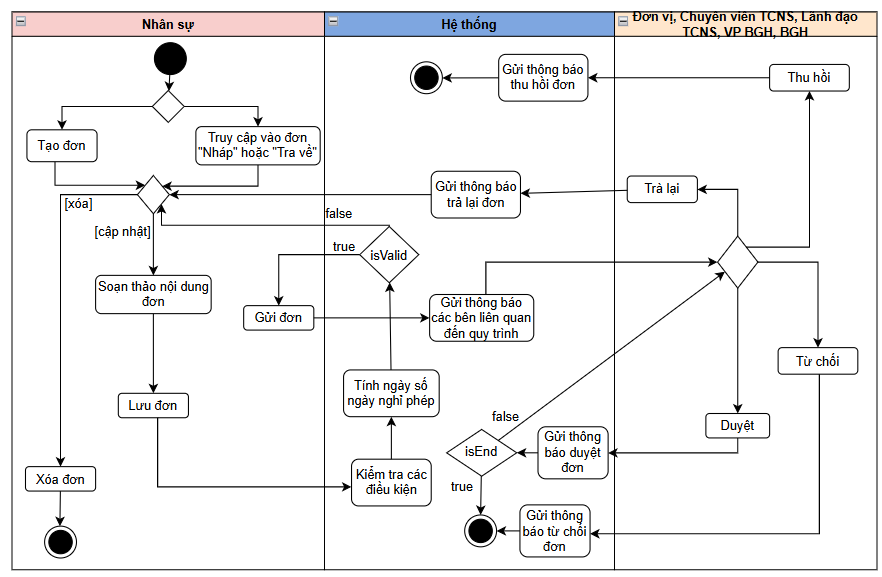
\includegraphics[width=\linewidth]{image/uml/leave_activity.png}
\caption{Biểu đồ hoạt động Quy trình nghỉ phép}
\label{fig:act_leave_submit}
\end{figure}

\subsubsection{Biểu đồ tuần tự}
Hình~\ref{fig:seq_leave_submit} minh họa UC-LEV-02: khởi tạo nháp, hoàn thiện dữ liệu và gửi vào quy trình chờ duyệt.

\begin{figure}[H]
\centering
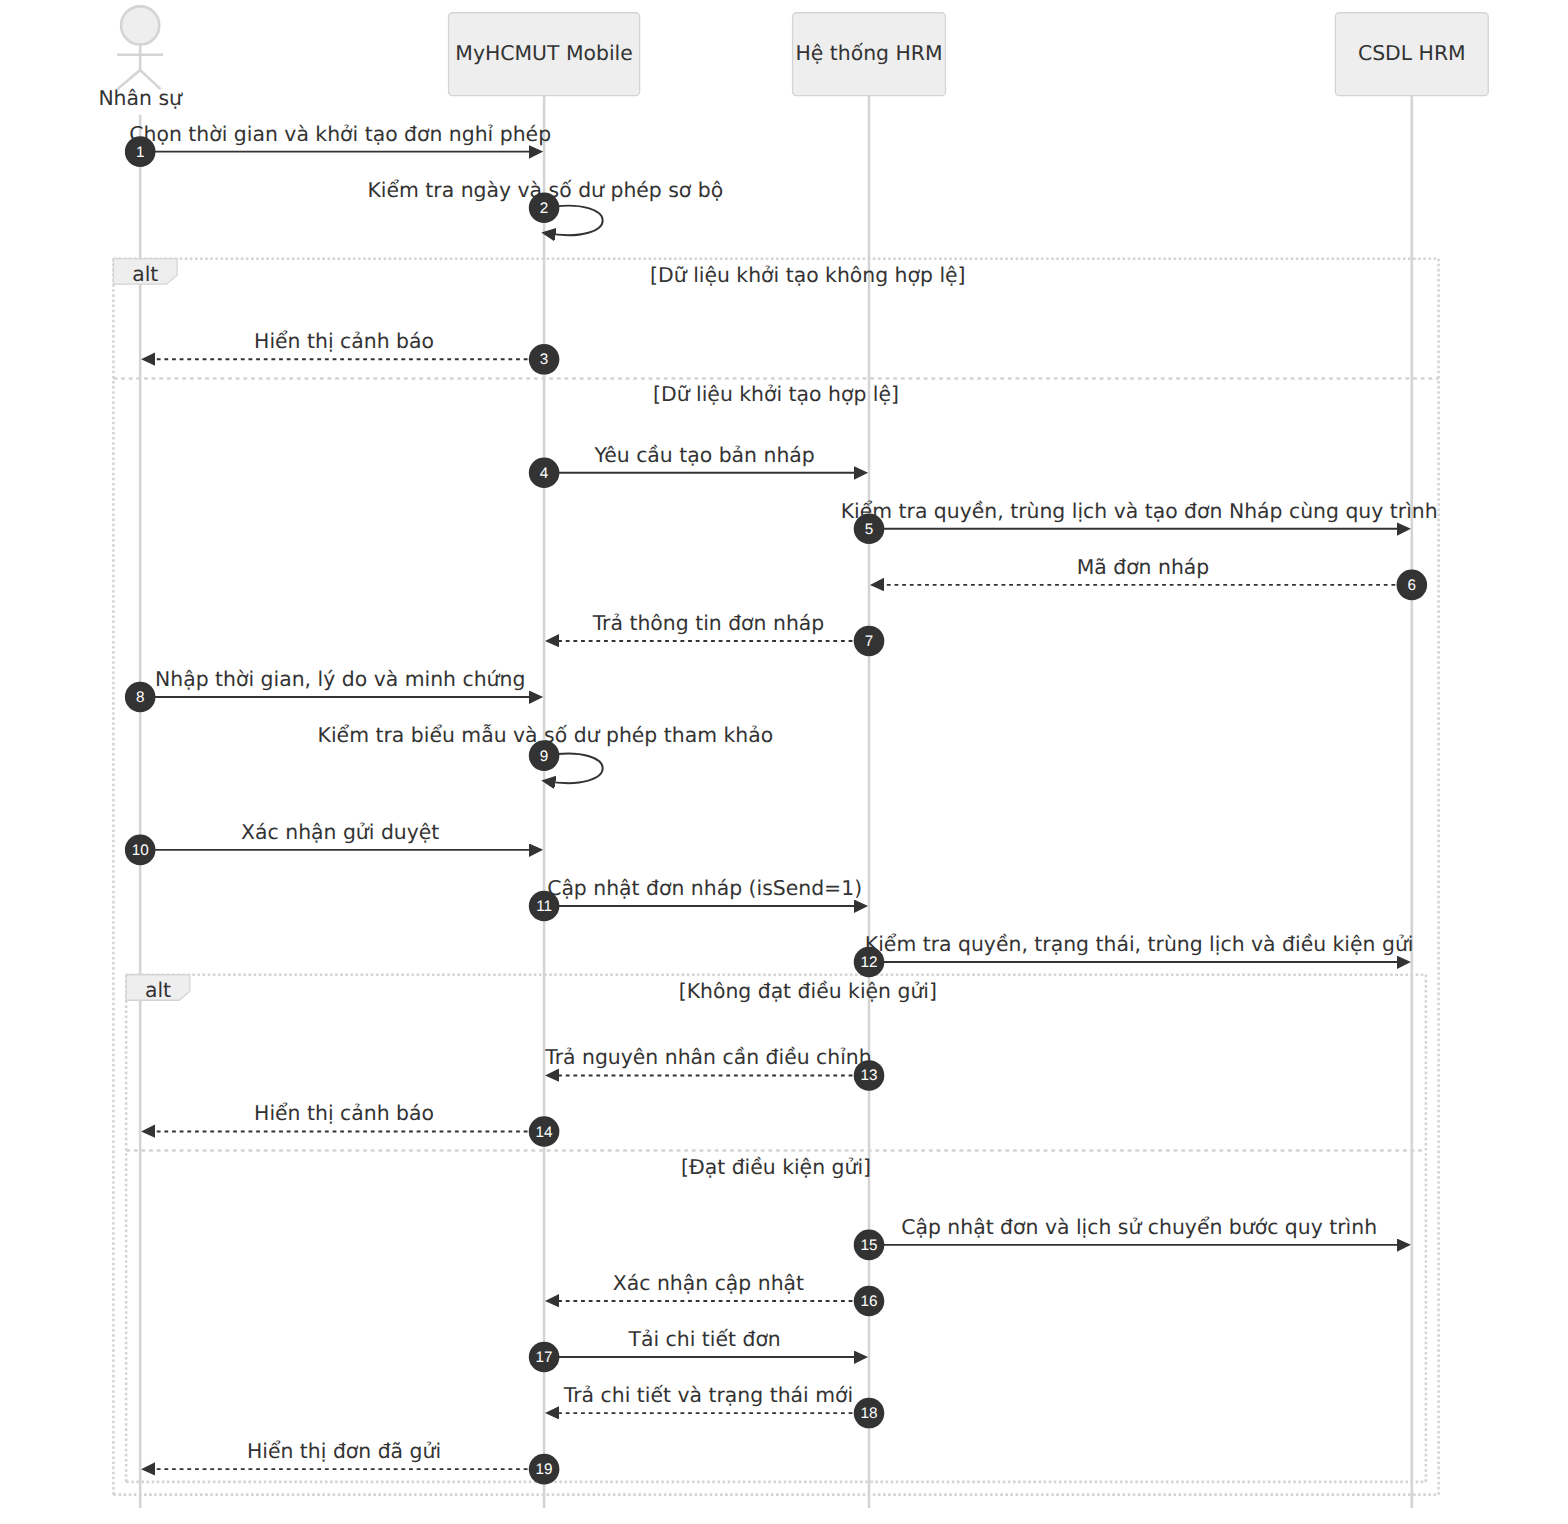
\includegraphics[width=\linewidth]{image/uml/seq_leave_submit.png}
\caption{Biểu đồ tuần tự Gửi yêu cầu nghỉ phép}
\label{fig:seq_leave_submit}
\end{figure}
